%\tikzstyle{charge}=[ball color=red!60]

\section*{Exercise Problems}

\begin{enumerate}

\item There are four charged objects: A, B, C, and D. Object A is charged
  positively. Object A is attracted to Object B. Object B is repelled from
  Object C. Object C is attracted to Object D. What are the charges on
  Objects B, C, and D?
  \begin{enumerate}
  \item B is negative, and C and D are positive.
  \item B and C are positive, and D is negative.
  \item B, C, and D are positive.
  \item B, C, and D are negative.
  \item B and C are negative, and D is positive.
  \end{enumerate}

\item An electron and a proton are separated by \SI{1.50e-10}\metre. If they
  are released, which one will accelerate at a greater rate, and what is the
  magnitude of that acceleration?
  \begin{enumerate}
  \item The electron; \SI{1.12e22}{\metre\per\second\squared}
  \item The proton;   \SI{1.12e22}{\metre\per\second\squared}
  \item The electron; \SI{6.13e18}{\metre\per\second\squared}
  \item The proton;   \SI{6.13e18}{\metre\per\second\squared}
  \item They both accelerate at the same rate:
    \SI{1.02e-8}{\metre\per\second\squared}
  \end{enumerate}

\item A carbon nucleus has 6 protons. What can be said about the electrostatic
  force between an orbital electron and the carbon nucleus?
  \begin{enumerate}
  \item The attractive force of the nucleus on the electron is greater than
    the force of the electron on the nucleus.
  \item The attractive force of the nucleus on the electron is less than the
    force of the electron on the nucleus.
  \item The attractive force of the nucleus on the electron is equal to the
    force of the electron on the nucleus.
  \item The repulsive force of the nucleus on the electron is equal to the
    force of the electron on the nucleus.
  \item The repulsive force of the nucleus on the electron is greater than
    the force of the electron on the nucleus.
  \end{enumerate}
  
\item Electric potential
  \begin{enumerate}
  \item is a vector quantity that depends on the direction of the electric
    field
  \item is a scalar quantity that depends on the magnitude and sign of
    charges in the vicinity
  \item is a scalar quantity that depends on the square of the distance
    from the charges in the vicinity
  \item is a vector quantity that depends on the sign of the charges in
    the vicinity
  \item is a vector quantity that must point from high to low potential
  \end{enumerate}
  
\item Which of the following statements is true of electric field and
  equipotential lines?
  \begin{enumerate}
  \item The electric field vector always points in the same direction as
    the equipotential lines.
  \item The electric field always points in the opposite direction of the
    equipotential lines.
  \item The electric field always points perpendicular to the
    equipotential lines.
  \item The electric field is always equal to the equipotential lines.
  \item Equipotential lines always form a circle around electric field
    lines.
  \end{enumerate}

  \begin{center}
    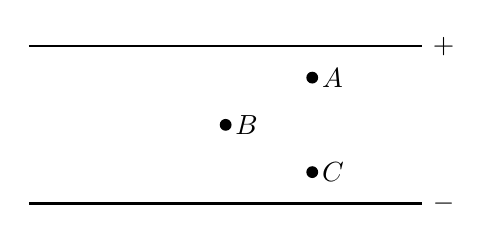
\begin{tikzpicture}
      \draw[thick] (0,2)--(5,2) node[right]{$+$};
      \draw[thick] (0,0)--(5,0) node[right]{$-$};
      \fill (3.6,1.6) circle (.075) node[right]{$A$};
      \fill (3.6,0.4) circle (.075) node[right]{$C$};
      \fill (2.5,1) circle (.075) node[right]{$B$};
    \end{tikzpicture}
    \end{center}
\item An electron is placed between two charged parallel plates at $A$,
  as shown above. It is then moved to $B$ and then to $C$. Which of the
  following statements are true:
  \begin{enumerate}[nosep,label=\Roman*.]
  \item The electrostatic force is greater at $A$ than at $B$.
  \item The work done from $A$ to $B$ to $C$ is the same as the work done from
    $A$ to $C$.
  \item The electrostatic force is the same at points $A$ and $C$.
  \item The electric field strength decreases as the electron is repelled
    upward.
  \end{enumerate}
  \begin{enumerate}
  \item I and II
  \item I and III
  \item II and III
  \item II and IV
  \item III and IV
  \end{enumerate}

%  %\item Explain what is meant by ``field'' and compare the properties of
%  %gravitational, electric, and magnetic forces in terms of particles affected,
%  %factors affecting the magnitude, and their relative strengths.
%
%  
%  \item A test charge of $+5.0$ \si{\micro\coulomb} experiences a force of
%  \SI{2.0e3}{\newton} [S] when placed at the midpoint of two oppositely
%  charge parallel plates. Assuming that the plates are electrically isolated
%  and have a distance of separation of 8.0 mm, what will be the
%  force experienced by a different charge of \SI{-2.0}{\micro\coulomb}, located
%  \SI{2.0}{\milli\metre} from the negative plate?
%  \vspace{\stretch1}
%  
%  %\item A positive charge of \SI{3.2e-5}{\coulomb} experiences a force of
%  %\SI{4.8}{\newton} to the right when placed in an electric field. What is the
%  %magnitude and direction of the electric field at the location of the charge?
%  %\vspace{1.1in}
%  
%  %\item What would be the electric field (magnitude and direction) of
%  %\SI{1.50}{\centi\metre} to the right of a charge of \SI{-6.5e-6}{\coulomb}? 
%
%  %\item A point charge has an excess of \SI{5.0e12}{C}. What would be the 
%  %electric potential at a distance of \SI{.50}{\metre} from the charge?
%  
%  \item A positively charged particle ($A$) is fixed in place, unable to
%  move. Another charged particle ($B$) is then brought near and released. 
%  \begin{enumerate}
%    \item Which way does $B$ move?
%    \item What happen to the force, acceleration, and velocity on the moving
%    particle as it moves?
%    \item What happens to the electric potential energy as B moves?
%  \end{enumerate}
%  (\emph{Some} of your answers will depend on the \emph{sign} of $B$;
%  you must specify all possibilities.)
  
\item What is the ratio of electrostatic to gravitational forces between an
  electron and a proton, i.e. $F_g/F_q$? (This question demonstrates the reason
  when dealing with atomic interactions, gravity can usually be ignored.)
  
  %\item Two 1 kg charges, each carry a charge of $+1$ C. What is the ratio
  %of gravitational force to the electrostatic force, 
  
\item In the Bohr model of the hydrogen atom, the electron moves in a circular
  orbit of radius $r$ around the proton.
  \begin{enumerate}
  \item Find an expression for the kinetic energy of the electron as a
    function of $r$. Show that at any distance $r$ the kinetic energy is
    negative one half the potential energy.
  \item Evaluate kinetic energy $K$, potential energy $U_q$ and the total
    energy $E=K+U_q$ in \underline{electron volts} for $r=\SI{0.529e-10}\metre$,
    the radius of the electron's orbit in hydrogen. %(The energy $|E|$ that must
    %be supplied to the hydrogen atom to remove the electron is called the
  \item What is the energy required to remove the electron from the atom? (This
    is called the \emph{ionization energy}.)
  \end{enumerate}

\item A small latex sphere experiences an electric force of
  \SI{3.6e-14}{\newton} when suspended halfway between a pair of large metal
  plates, which are separated by \SI{48.}{\milli\metre}. There is just enough
  electric force to balance the force of gravity on the sphere.
  \begin{enumerate}
  \item What is the mass of the sphere?
  \item What is the potential difference between the plates, given that the
    charge on the sphere is \SI{4.8e-19}\coulomb?
  \end{enumerate}
  
\item Physicist Robert Millikan used an \emph{oil drop experiment} to discover
  the elementary charge, by suspending charged oil drops inside a known
  electric field between two parallel plates. In an experiment replicating
  Millikan's oil drop experiment, a pair of parallel plates placed
  \SI{1.96}{\milli\metre} apart and the top plate is positive. When the
  potential difference across the plates is \SI{240}\volt, an oil drop of mass
  \SI{2.00e-14}{\kilo\gram} gets suspended between the plates.
  \begin{enumerate}
  \item Draw a free-body diagram for the charge.
  \item What is the charge on the oil drop?
  \item Is there an excess or deficit of electrons on the oil drop? Explain.
  \item How many electrons are in excess or deficit?
  \end{enumerate}

%  \item Using your vast knowledge of electric fields, draw diagrams showing
%  the electric field around the following configurations:
%
%  \vspace{.15in}
%  \begin{minipage}{.46\textwidth}
%    (a) A single stationary positive charge
%    \vspace{.7in}
%    \begin{center}
%      {\tikz\draw[thick] circle(.2) node{$+$};}
%    \end{center}
%    \vspace{.7in}
%  \end{minipage}
%  \begin{minipage}{.475\textwidth}
%    (b) Between two parallel plates
%    \vspace{.15in}
%    \begin{center}
%      \begin{tikzpicture}[thick]
%        \draw (0,2)--(5,2) node[midway,above]{$-\;-\;-\;-\;-\;-\;-\;-\;-\;-$};
%        \draw (0,0)--(5,0) node[midway,below]{$+\;+\;+\;+\;+\;+\;+\;+\;+\;+$};
%      \end{tikzpicture}
%    \end{center}
%    \vspace{.15in}
%  \end{minipage}
%  
%  \begin{minipage}{.46\textwidth}
%    (c) Three point charges
%    \vspace{.7in}
%    \begin{center}
%      \begin{tikzpicture}[thick]
%        \draw circle(.2) node{$+$};
%        \draw (0,2) circle(.2) node{$+$};
%        \draw (4,1) circle(.2) node{$-$};
%      \end{tikzpicture}
%    \end{center}
%    \vspace{.7in}
%  \end{minipage}
%  \begin{minipage}{.475\textwidth}
%    (d) Point charge and a thin rod with uniform positive charge
%    \vspace{.3in}
%    \begin{center}
%      \begin{tikzpicture}[thick]
%        \draw circle(.2) node[midway]{$-$};
%        \draw (4,-2) rectangle (4.3,2);
%      \end{tikzpicture}
%    \end{center}
%    \vspace{.3in}
%  \end{minipage}
%   

%  %\item How is the electric field between parallel plates different from
%  %the electric field of a point charge? 
%
\item An electron starts at rest and accelerates through an electric field
  established by a set of parallel plates with a potential difference of
  \SI{35}\volt.
  \begin{enumerate}
    % The original version has the electron hitting the negative plate, which
    % is pretty impossible consider the repelling force.
  \item What is the speed of the electron the instant before it hits the
    positive plate?

  \item Instead of hitting the postive plate, the electron, travelling East,
    escapes the parallel plates through a small hole and enters a magnetic
    field of \SI{.75}{\tesla} directed downward.  What will be the magnetic
    force (magnitude and direction) on the charge?
    
  \item Once the electron has entered the magnetic field, it is in circular
    motion. What is the radius of the electron's circular path? 
  \end{enumerate}

\item Charge $A(+6.0\si{\micro\coulomb})$ is separated \SI{10.0}{\centi\metre}
  from charge $B(-2.0\si{\micro\coulomb})$. At what location along the line
  that passes through the two charges will the total electric potential be zero?

  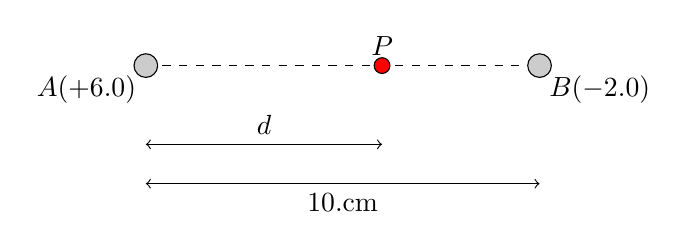
\begin{tikzpicture}[scale=5]
    \draw[dashed](0,0)--(1,0);
    \draw[<->](0,-.2)--(.6,-.2) node[midway,above]{$d$};
    \draw[<->](0,-.3)--(1,-.3) node[midway,below]{\SI{10.}{cm}};
    \draw[fill=gray!40] circle(.03)
    node[below left] {$A(+6.0\si{\micro\coulomb})$};
    \draw[fill=gray!40](1,0) circle(.03)
    node[below right]{$B(-2.0\si{\micro\coulomb})$};
    \draw[fill=red](.6,0) circle(.02) node[above]{$P$};
  \end{tikzpicture}

\item The potential gradient between two parallel plates
  \SI{2.}{\centi\metre} apart is \SI{2.0e3}{\volt\per\metre}.
  \begin{enumerate}
  \item What is the potential difference between the plates?
  \item What is the electric field intensity between the plates?
  \end{enumerate}
  
\item An \emph{electric dipole} is a pair of charged particles with equal
  but opposite charges. One such example is shown in the diagram below.
  Two particles with charges $+12$ \si{\micro\coulomb} and
  \SI{-12}{\micro\coulomb} are \SI{1.0}{\milli\metre} apart along the $x$-axis.
  What is the electric field (magnitude and direction) at $P$?
  
  \begin{tikzpicture}[scale=2.8]
    \draw[axes] (-1,0)--(1,0) node[right]{$x$};
    \draw[axes] (0,-.5)--(0,.75) node[above]{$y$};
    \shade[poscharge] (-.5,0) circle(.05)
    node[below left]{\SI{-12}{\micro\coulomb}};
    \shade[poscharge] (.5,0) circle(.05)
    node[below right]{+\SI{12}{\micro\coulomb}};
    \fill (0,.5) circle(.015) node[right]{$P$};
    \draw[thick,<->] (0,.475)--(0,0) node[midway,right]{0.50 mm};
    \draw[thick,<->] (0,-.2)--(.5,-.2) node[midway,below]{0.50 mm};
    \draw[thick,<->] (-.5,-.4)--(.5,-.4) node[midway,below]{1.0 mm};
    \draw[dashed] (.5,-.05)--(.5,-.45);
    \draw[dashed] (-.5,-.05)--(-.5,-.45);
  \end{tikzpicture}

\item Two identical spheres of mass $m$ are suspended from a common point by
  threads of length $\ell$. When each sphere carries a charge $q$, each thread
  makes an angle $\phi$ with the vertical.
  \begin{enumerate}
  \item Express charge $q$ in terms of $\theta$, $m$, $L$ and any appropriate
    fundamental constants.
  \item Compute $q$ if $m=\SI{10}\gram$, $\ell=\SI{50}{\centi\metre}$ and
    $\phi=\ang{10}$
  \end{enumerate}
  \begin{tikzpicture}
    \fill[yellow!20] (-1.5,0) rectangle(1.5,.15);
    \draw[thick] (-1.5,0)--(1.5,0);
    \draw[dashed,very thick] (0,0)--(0,-4);
    \draw[axes] (0,-2.5) arc (270:285:2.5) node[midway,below]{$\phi$};
    \draw[axes] (0,-2.5) arc (270:255:2.5) node[midway,below]{$\phi$};
    \begin{scope}[rotate=15]
      \draw[very thick] (0,0)--(0,-3.5) node[midway,right]{$\ell$};
      \shade[poscharge] (0,-3.5) circle (.2) node[right=8]{$Q$};
    \end{scope}
    \begin{scope}[rotate=-15]
      \draw[very thick] (0,0)--(0,-3.5) node[midway,left]{$\ell$};
      \shade[poscharge] (0,-3.5) circle (.25) node[left=8]{$Q$};
    \end{scope}
  \end{tikzpicture}

\item Five equal charges $Q$ are equally spaced on a semicircle or radius $R$
  as shown in the figure below. Find the force on a charge $q$ located at the
  centre of the semicircle.
  
  \begin{tikzpicture}
    \draw[axes] (0,-1.75)--(0,2.3) node[above]{$y$};
    \draw[axes] (-2.5,0)--(1.5,0) node[right]{$x$};
    \draw[->,rotate=150] (0,0)--(1.75,0) node[midway,above]{$R$};
    \draw(0,1.75) arc (90:270:1.75);
    \foreach \x in {0,45,...,180}
    \shade[balloon1,rotate=\x] (0,1.75) circle(.2) node[left=5]{$Q$};
    \shade[balloon2] circle (.12) node[below right]{$q$};
  \end{tikzpicture}

%  \item Four charges are at the corners of a square centred at the origin
%  as follows: $q$ at $(-a,+a)$, $2q$ at $(+a,+a)$, $3q$ at $(+a,-a)$, and
%  $6q$ at $(-a,-a)$.
%  \begin{enumerate}
%    \item Find the electric potential at the origin
%    \item If a 5th charge of $q$ with mass $m$ is placed at the origin and
%    released, what would be its speed when it is a great distance from the
%    origin?
%  \end{enumerate}
%  \vspace{\stretch1}
%
%  %\item A charge $q$ is at $x=0$ and a charge $-3q$ is at $x=1$.
%  %\begin{enumerate}
%  %  \item Find $V(x)$ for a general point along the $x$ axis, and sketch $V(x)$
%  %  vs.\ $x$ in the space below. (Hint: the potential at $x=0$ and $x=1$ are
%  %  undefined because they are asymptotes.)
%  %  \begin{center}
%  %    \vspace{-.05in}
%  %    \begin{tikzpicture}[scale=.7]
%  %      \draw[gray!50,thin] grid(16,12);
%  %      \draw[thick,->](0,6)--(16.5,6) node[right]{$x$};
%  %      \draw[thick,->](8,0)--(8,12.5) node[above]{$V$};
%  %    \end{tikzpicture}
%  %  \end{center}
%  %  \item Find the points on the $x$ axis where the potential is zero.
%  %\end{enumerate}
\end{enumerate}
